% -*- latex -*-
% FILE: "/home/evmik/jobs/wm/2012_spring_Analog_Electronics_252/final_exam/questions/thevenin_parameters_of_a_circuit.tex"
% LAST MODIFICATION: "Mon, 30 Apr 2012 23:10:08 -0400 (evmik)"
% (C) 2011 by Eugeniy Mikhailov, <evgmik@gmail.com>
% $Id:$

\question{}
	Consider the circuit shown below \\
	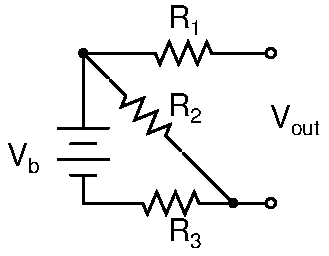
\includegraphics[width=0.25\textwidth]{./schematics/resistors_net}\\
	Where $R_1$=8~k$\Omega$, $R_2$=6~k$\Omega$, $R_3$=3~k$\Omega$, and
	the battery voltage $V_b=18$~V.\\
	{\bf Hint 1:} For solving below problems, it is helpful to mentally connect a dummy load and express {\bf
	symbolically} the $V_{out}$ vs $I_{out}$ for different $R_L$.
	{\bf Hint 2:} There is a faster way.
	\begin{parts}
		\part[8]
		What is the Th\'{e}venin voltage  of this circuit?

		\vskip 2.0in
		$V_{th}=$
		\part[8]
		What is the Th\'{e}venin resistance  of this circuit?

		\vskip 2.0in
		$R_{th}=$
		\part[5]
		If someone connected a load with resistance $R_L$=1~k$\Omega$ 
		what is the power dissipated by this load?

		\vskip 0.5in
		$P_{L}=$
		\part[4]
		While the same load connected to the circuit what is the total power
		dissipated by all resistors (excluding the load)  of the circuit
		network.


		\vskip 0.5in
		$P_{tot}=$
	\end{parts}
	\pagebreak

